
%(BEGIN_QUESTION)
% Copyright 2010, Tony R. Kuphaldt, released under the Creative Commons Attribution License (v 1.0)
% This means you may do almost anything with this work of mine, so long as you give me proper credit

The temperature inside this chemical reactor vessel is controlled by a temperature control valve (TV) at top, and is measured by redundant temperature transmitters sending their signals through a ``high-select'' function:

$$\includegraphics[width=15.5cm]{i04595x01.eps}$$

Explain what will happen (and why!) if a technician temporarily disconnects temperature transmitter 29c from its sensing element in such a way that the transmitter outputs a {\it low} signal.

\vskip 20pt \vbox{\hrule \hbox{\strut \vrule{} {\bf Suggestions for Socratic discussion} \vrule} \hrule}

\begin{itemize}
\item{} Suppose these were FOUNDATION Fieldbus temperature transmitters rather than analog temperature transmitters.  Would the effects of disconnecting TT-29c from the Fieldbus segment be the same?  Why or why not?
\end{itemize}

\underbar{file i04595}
%(END_QUESTION)





%(BEGIN_ANSWER)

There probably will not be any effect at all from doing this, as the high-select function only sends the {\it highest} temperature signal to the controller.  Of course, this means if TE-29c happened to sense a hotter temperature than the other elements and then was disconnected, the control system would see a small drop in temperature (as it now selected the next-highest transmitter's signal) and would send a bit more cooling water to the jacket as designed.

%(END_ANSWER)





%(BEGIN_NOTES)


%INDEX% Basics, control loop troubleshooting: determining effect of specified fault(s)
%INDEX% Process: reactor temperature control (generic)

%(END_NOTES)

